\section{Step 2 - Drawing Spheres}
\subsection{Drawing spheres from points}
Our first sample which adds some geometric objects is pretty simple.
Execute {\tt Step2\_1.py}, click on menu {\tt Draw} menu-item  {\tt draw sphere 1} and after that click on menu {\tt Draw} menu-item  {\tt draw sphere 2} to see the screen shown in figure~\ref{STEP_2_1_SCREEN}.
If you click on menu {\tt Erase} menu-item  {\tt erase all} the whole canvas will be erased.
% +++++++++++++++++++++++++++++++++++++++++++++++++++++++++++++++++++++++ 
% +++ Bild: Step 2_1 ++++++++++++++++++++++++++++++++++++++++++++++++++++
% +++++++++++++++++++++++++++++++++++++++++++++++++++++++++++++++++++++++ 
\begin{figure}[h]
\begin{center}
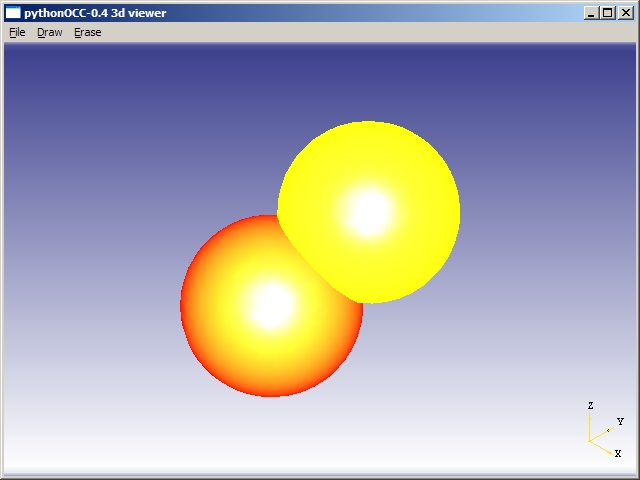
\includegraphics[height=8.5cm,width=11.3cm]{Step2_1.jpg}
\end{center}
\caption[Screenshot of Step2\_1]{\label{STEP_2_1_SCREEN}Screenshot of Step2\_1}
\end{figure}

Time to learn navigating with the mouse!
Display both spheres utilising the menu.
Do the following:
\begin{enumerate}
\item Move the mouse into the screen, press the left mouse button and hold it
		down.
		Move the mouse with the left mouse button pressed down.
		See that the coordinate system in the right corner at the bottom and the
		objects turn according to your mouse moves.
		So moving the mouse with the left mouse button held down rotates the 
		model.
		This cannot be seen with one sphere because a sphere looks the same from
		every side. 
\item Press the middle mouse button and move the mouse. 
		This causes a translation of the spheres.
\item Hold down the right mouse button and move the mouse to the left.
		The objects moves away from you.
		Now move the mouse to the right with the right mouse button held down.
		The objects come closer.
\end{enumerate}

Let's have a look at the code.
Listing~\ref{LISTING_STEP2_1_PY_A} shows how the menu and menu-items were changed to make the new funcionality available in the graphical use interface.
\begin{python}[moreemph={[4], 46, 48},caption={Step2\_1.py - Extending the menu},label=LISTING_STEP2_1_PY_A]
...
    # This is the place where we hook our functionality to menus
    # ----------------------------------------------------------
    add_menu('File')
    add_function_to_menu('File',  exit)
    add_menu('Draw')
    add_function_to_menu('Draw', draw_sphere_1)
    add_function_to_menu('Draw', draw_sphere_2)
    add_menu('Erase')
    add_function_to_menu('Erase', erase_all)
...    
\end{python}
As you can see in listing~\ref{LISTING_STEP2_1_PY_B} there are two functions {\tt draw\_sphere\_1} and {\tt draw\_sphere\_2} added under menu {\tt Draw}.
The new menu {\tt Erase} is bound to function {\tt erase\_all}.
These functions are presented in listing~~\ref{LISTING_STEP2_1_PY_B}.
It should also be noted that we have to add two additional modules {\tt OCC.gp} and {\tt OCC.BRepPrimAPI}.
%
\begin{python}[moreemph={[4], 46, 48},caption={Step2\_1.py - Extending the functionality},label=LISTING_STEP2_1_PY_B]
# =============================================================================
# Packages to import
# =============================================================================
import OCC.Display.SimpleGui 
import sys
from OCC import VERSION
from OCC.Display.wxDisplay import wxViewer3d
import OCC.gp 
import OCC.BRepPrimAPI 

# =============================================================================
# Functions called from some menu-items
# =============================================================================
def draw_sphere_1(event=None):
    # create sphere
    Radius = 50.0
    # The sphere center
    X1 = 0.0
    Y1 = 0.0
    Z1 = 0.0
    # create OCC.gp.gp_Pnt-Point from vector
    Point = OCC.gp.gp_Pnt( X1, Y1, Z1 )     
    MySphere = OCC.BRepPrimAPI.BRepPrimAPI_MakeSphere( Point, Radius )  
    MySphereShape = MySphere.Shape()
    display.DisplayColoredShape( MySphereShape , 'RED' ) 

def draw_sphere_2(event=None):
    # create sphere
    Radius = 50.0
    # The sphere center
    X1 = 25.0
    Y1 = 50.0
    Z1 = 50.0
    # create OCC.gp.gp_Pnt-Point from vector
    Point = OCC.gp.gp_Pnt( X1, Y1, Z1 )     
    MySphere = OCC.BRepPrimAPI.BRepPrimAPI_MakeSphere( Point, Radius )  
    MySphereShape = MySphere.Shape()
    display.DisplayColoredShape( MySphereShape , 'YELLOW' ) 

def erase_all(event=None):
    display.EraseAll()
...    
\end{python}
A sphere is a so called primitive.
Boxes, tori, wedges, cylinders and cones are other primitives which are also availble in {\tt pythonOCC}.
To make use of these primitives we have to import {\tt OCC.BRepPrimAPI}.
In this course we will generate a lot of primitives so you can see how it works.
It should be noted that there are different constructors available for single primitives.
Please refer to the {\tt pythonOCC}~\cite{PYTHON_OCC_DOCU} documentation to see how these are constructed.
Sometimes consulting the C++ documentation of Open~Cascade~\cite{OPENCASCADE_ORG} is also be helpful.
In addition the {\it Modelling Algorithms Users Guide} which is available at the Open~Cascade web-site too offers additional information.
The latter does not contain every possibility so I recommend to read the documentation in html.

If we want to create and draw a primitive we always perform three steps.
\begin{enumerate}
\item Generate the primitive utilzing a constructor like \\ 
		{\tt MySphere=OCC.BRepPrimAPI.BRepPrimAPI\_MakeSphere(Point,Radius)}
\item Create the shape of the primitive\footnote{Until now I did not find out why this has to be done and what exactly is the difference of the primitive and its shape. But believe me we are able to make use of {\tt pythonOCC} for our visualization purposes without that knowledge. As soon as I understand the background I will update the document. Thomas Paviot recommended to read 
Roman Lygin's blog \href{http://opencascade.blogspot.com/2009/02/topology-and-geometry-in-open-cascade.html}{http://opencascade.blogspot.com/2009/02/topology-and-geometry-in-open-cascade.html} especially the pages dedicated to the topology data model. Thomas also announced some document concerning that topic.
}\\
		{\tt MySphereShape = MySphere.Shape()}
\item Display the shape\\
		{\tt display.DisplayColoredShape( MySphereShape , 'YELLOW' )}
\end{enumerate}

The constructor used in our code receives a variable {\tt Point} and a variable  {\tt Radius}.
{\tt Radius} is obviously just a floating point value but {\tt Point} is something that has to be created by\\
{\tt Point = OCC.gp.gp\_Pnt( X1, Y1, Z1 ) }\\
where {\tt X1}, {\tt X2} and {\tt X3} are floating point values.
Module {\tt OCC.gp} contains definitions of different geometric objects like points, circles, axes, directions and so on which are accepted by {\tt pythonOCC}.
The natural way to define a sphere is to specify a point at the center and a radius.
Because we are talking to {\tt pythonOCC} we have to enter the point in a way  {\tt pythonOCC} understands and thats in this case done by the specification of a {\tt OCC.gp.gp\_Pnt} object\footnote{In {\tt pythonOCC} objects carry their module names as a prefix. This helps if you have to read samples containing functions imported via {\tt from some\_module import~*}. Simply look at the prefix and you know the home module of the object.}.
%
\subsection{Drawing spheres from Scipy arrays}
At this point it is time for {\tt Scipy} to enter the scene.
{\tt Scipy} offers you great functionality for doing geometrical computations.
{\tt pythonOCC} and {\tt Scipy} are a great team which can easily be combined.

So have a look at {\tt Step2\_2.py} and see that we changed the beginning of the code like shown in listing~\ref{LISTING_STEP2_2_PY_A}
\begin{python}[moreemph={[4], 46, 48},caption={Step2\_1.py - Involve Scipy},label=LISTING_STEP2_2_PY_A]
# =============================================================================
# Packages to import
# =============================================================================
import OCC.Display.SimpleGui 
import sys
from OCC import VERSION
from OCC.Display.wxDisplay import wxViewer3d
import OCC.gp 
import OCC.BRepPrimAPI 
import scipy
# =============================================================================
# Functions generating primitives from Scipy arrays
# =============================================================================
def sphere_from_vector_and_radius(  vector, 
                                    radius ):
    '''
    Creates a sphere from a scipy vector and a radius

    @param vector: center of a sphere as a scipy array
    @type  vector: array(3,1)
    @param radius: radius of the sphere
    @type  radius: scalar
    '''
    # write the components of vector in float values
    X1 = float( vector[ 0, 0] )
    Y1 = float( vector[ 1, 0] )
    Z1 = float( vector[ 2, 0] )
    # create OCC.gp.gp_Pnt-Point from vector
    Point = OCC.gp.gp_Pnt( X1, Y1, Z1 )
    # create sphere
    sphere = OCC.BRepPrimAPI.BRepPrimAPI_MakeSphere( Point, radius )
    # retrurn the sphere
    return sphere 

# =============================================================================
# Functions called from some menu-items
# =============================================================================
def draw_sphere_1(event=None):
    # create sphere
    Radius = 50.0
    # The sphere center as a Scipy array - 3 rows, one column
    # Note we use the scipy.zeros function
    PointZeroArray = scipy.zeros((3,1), dtype=float)
    MySphere = sphere_from_vector_and_radius(   PointZeroArray, 
                                                Radius )
    MySphereShape = MySphere.Shape()
    display.DisplayColoredShape( MySphereShape , 'RED' ) 

def draw_sphere_2(event=None):
    # create sphere
    Radius = 50.0
    # The sphere center as a Scipy array - 3 rows, one column
    MyPointAsArray = scipy.array([25.0, 50.0, 50.0])
    MyPointAsArray = scipy.reshape(MyPointAsArray,(3,1))
    MySphere = sphere_from_vector_and_radius(   MyPointAsArray, 
                                                Radius )
    MySphereShape = MySphere.Shape()
    display.DisplayColoredShape( MySphereShape , 'YELLOW' ) 
...    
\end{python}
If you run {\tt Step2\_2.py} you get the same result as you got from {\tt Step2\_1.py}.
The difference between these programs lies in the construction of the sphere.
In {\tt Step2\_1.py} we defined three floating point values and generated a {\tt \tt OCC.gp.gp\_Pnt} object.
In {\tt Step2\_2.py} a {\tt Scipy} array is used for that purpose.

Functions {\tt draw\_sphere\_1} and  {\tt draw\_sphere\_2} are creating an array.
The first one does this by calling {\tt scipy.zeros} the latter on by {\tt scipy.array} so you can realize that both options work.

Now function {\tt sphere\_from\_vector\_and\_radius} is called.
Here we construct the sphere.
Experience showed that it is always a good idea to cast the content of the array in the way shown below.
\begin{python}
...    
    # write the components of vector in float values
    X1 = float( vector[ 0, 0] )
    Y1 = float( vector[ 1, 0] )
    Z1 = float( vector[ 2, 0] )
...    
\end{python}
